
% This LaTeX was auto-generated from MATLAB code.
% To make changes, update the MATLAB code and republish this document.

\documentclass{article}
\usepackage{graphicx}
\usepackage{color}

\sloppy
\definecolor{lightgray}{gray}{0.5}
\setlength{\parindent}{0pt}

\begin{document}

    
    
\subsection*{Contents}

\begin{itemize}
\setlength{\itemsep}{-1ex}
   \item Inputs
   \item Motor Torque-Speed
   \item Gear Ratio Target (minimization)
   \item Gears
   \item Gear Ratio (Overall)
   \item Shaft Torque and Speed Estimation
   \item Operating Gear Forces, Torques and Diameters
   \item Stresses
   \item Torque Calculation
   \item Shaft A BMD
   \item Shaft B BMD
   \item Shaft C BMD
   \item BMD Tables
   \item Endurance Limits
   \item Test
\end{itemize}
\begin{verbatim}
clear
clc
resloution = 0.001;
\end{verbatim}


\subsection*{Inputs}

\begin{verbatim}
%All in standard SI units unless noted
OperatingVoltage = 40                                               %V
TorqueConstant = 8.474E-3                                           %N.m/A
VoltageConstant = 1125                                              %RPM/V
ArmatureResistance = 0.072                                          %Ohms
reqOutputSpeed = 575                                                %RPM
reqOutputTorque = 55                                                %N.m
Efficiency = 90/100
Duty = 2000                                                         %Hours

%Gear Specs
PressureAngle = 20*pi/180                                           %Rad
FaceWidth = [1.5, 1.25, 1, 0.75, 0.5, 0.25, 0.188, 0.125]           %inch
DiametralPitch = [8, 10, 12, 16, 20, 24, 32, 48]                    %teeth/inch
DiametralPitchSelected = 20;
k = 1                                                               %Teeth Depth (1 = full)

%Number of teeth variables:
P1 = 16
N1 = 70
P2 = 16
N2 = 70
\end{verbatim}

        \color{lightgray} \begin{verbatim}
OperatingVoltage =

    40


TorqueConstant =

    0.0085


VoltageConstant =

        1125


ArmatureResistance =

    0.0720


reqOutputSpeed =

   575


reqOutputTorque =

    55


Efficiency =

    0.9000


Duty =

        2000


PressureAngle =

    0.3491


FaceWidth =

  Columns 1 through 7

    1.5000    1.2500    1.0000    0.7500    0.5000    0.2500    0.1880

  Column 8

    0.1250


DiametralPitch =

     8    10    12    16    20    24    32    48


k =

     1


P1 =

    16


N1 =

    70


P2 =

    16


N2 =

    70

\end{verbatim} \color{black}
    

\subsection*{Motor Torque-Speed}

\begin{verbatim}
%point 1:
NoLoadSpeed = VoltageConstant*OperatingVoltage;
NoLoadTorque = 0;
%point 2:
StallTorque = TorqueConstant*OperatingVoltage/ArmatureResistance;
StallSpeed = 0;

%determine Torque-speed graph
points = [StallSpeed, StallTorque;
          NoLoadSpeed, NoLoadTorque];
polynomialDegree = length(points)-1;

%fit a polynomial to the two data points
MotorLine = polyfit(points(:,1),points(:,2),polynomialDegree);

%generate figure
f1 = figure('Renderer', 'painters', 'Position', [10 10 1200 300])
subplot(1,3,1)
plot([StallSpeed:NoLoadSpeed], polyval(MotorLine,[StallSpeed:NoLoadSpeed]))
hold on
title("Motor Torque-Speed")
xlabel("Motor Speed (rpm)")
ylabel("Motor Torque (N.m)")
hold off
\end{verbatim}

        \color{lightgray} \begin{verbatim}
f1 = 

  Figure (1) with properties:

      Number: 1
        Name: ''
       Color: [0.9400 0.9400 0.9400]
    Position: [10 10 1200 300]
       Units: 'pixels'

  Use GET to show all properties

\end{verbatim} \color{black}
    
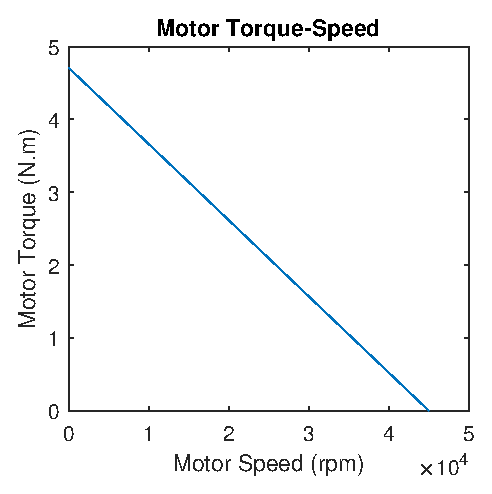
\includegraphics [width=4in]{main_01.eps}


\subsection*{Gear Ratio Target (minimization)}

\begin{verbatim}
%setup equation to determine optimal ratio
syms r
eqn = MotorLine(1)*reqOutputSpeed*r^2 + MotorLine(2)*r == reqOutputTorque;
soln = double(solve(eqn,r))

%solve equation for tearget ratio
ratioTarget = soln(1);

%determine line for the target ratio
TargetLine = [MotorLine(1)*ratioTarget^2, MotorLine(2)*ratioTarget];

%generate figure
subplot(1,3,2)
plot([StallSpeed/ratioTarget: NoLoadSpeed/ratioTarget], polyval(TargetLine,[StallSpeed/ratioTarget: NoLoadSpeed/ratioTarget]))
hold on
plot(reqOutputSpeed, reqOutputTorque,'*')
title(["Drill Torque-Speed (Target), m = ", ratioTarget])
xlabel("Drill Speed (rpm)")
ylabel("Drill Torque (N.m)")
legend("Drill Output", "Given Requirement")
hold off
\end{verbatim}

        \color{lightgray} \begin{verbatim}
soln =

   14.2933
   63.9676

\end{verbatim} \color{black}
    
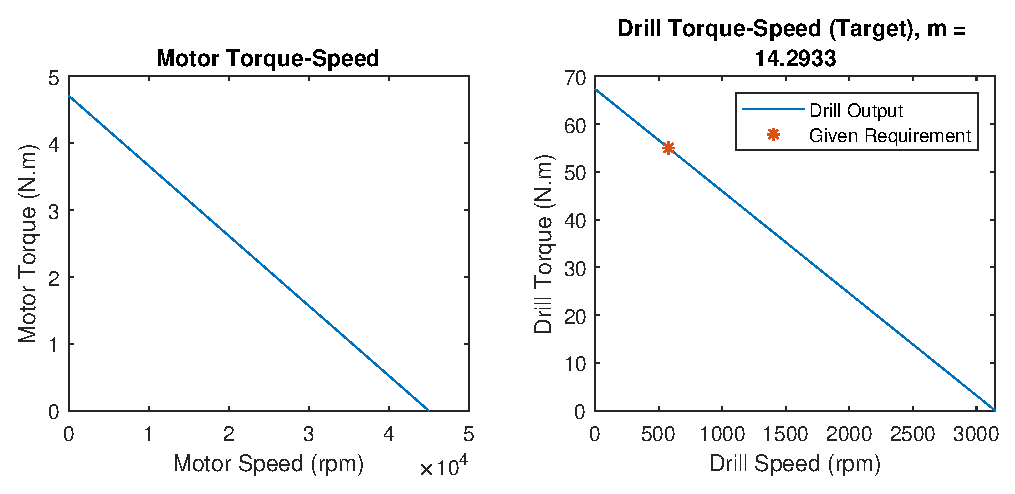
\includegraphics [width=4in]{main_02.eps}


\subsection*{Gears}

\begin{verbatim}
m1actual = N1/P1;
m2actual = N2/P2;
ratio = m1actual*m2actual;

%limits:
%pinions
P1l = ceil((2*k*(m1actual+(m1actual^2+(1-2*m1actual)*(sin(PressureAngle))^2)^0.5))/((1+2*m1actual)*(sin(PressureAngle))^2));
P2l = ceil((2*k*(m2actual+(m2actual^2+(1-2*m2actual)*(sin(PressureAngle))^2)^0.5))/((1+2*m2actual)*(sin(PressureAngle))^2));

%gear Limits
N1l = floor(((P1l^2)*(sin(PressureAngle)^2)-4*k^2)/(4*k-2*P1l*sin(PressureAngle)^2));
N2l = floor(((P1l^2)*(sin(PressureAngle)^2)-4*k^2)/(4*k-2*P2l*sin(PressureAngle)^2));

%generate ratio table
TRatio = table(P1, P1l, N1, N1l, m1actual, P2, P2l, N2, N2l, m2actual, ratio)

%old ratio determiner
%{
if(m1*P1l > N1l)
    N1 = N1l;   %Gear Ratio m is too large
    disp("Ratio m1 Too Large, increasing P1")
    P1l = P1l+1;
    N1 = floor(m1*P1l);
else
    N1 = floor(m1*P1l);
end

if(m2*P2 > N2l);
    N2 = N2l;    %Gear Ratio m is too large
    disp("Ratio m2 Too Large, increasing P2")
    P2 = P2+1;
    N2 = floor(m2*P2);
else
    N2 = floor(m2*P2);
end

%}
\end{verbatim}

        \color{lightgray} \begin{verbatim}
TRatio =

  1�1�7 table

    P1    P1l    N1    N1l    m1actual    P2    P2l    N2    N2l    m2actual    ratio 
    __    ___    __    ___    ________    __    ___    __    ___    ________    ______

    16    16     70    101     4.375      16    16     70    101     4.375      19.141

\end{verbatim} \color{black}
    

\subsection*{Gear Ratio (Overall)}

\begin{verbatim}
outputTorque = [0];
outputSpeed = [0];

%Adjust line with ratio
RealLine = [MotorLine(1)*ratio^2, MotorLine(2)*ratio];

for x = [StallSpeed:NoLoadSpeed]
   outputSpeed = [outputSpeed, x/ratio];
   outputTorque = [outputTorque, polyval(RealLine,x/ratio)];
end
outputSpeed = outputSpeed(2:end);
outputTorque = outputTorque(2:end);

%generate figure
subplot(1,3,3)
plot(outputSpeed, outputTorque)
hold on
plot(reqOutputSpeed,reqOutputTorque,'*')
title(["Drill Torque-Speed (Actual) m = ", ratio])
xlabel("Drill Speed (rpm)")
ylabel("Drill Torque (N.m)")
legend("Drill Output", "Given Requirement")
hold off
\end{verbatim}

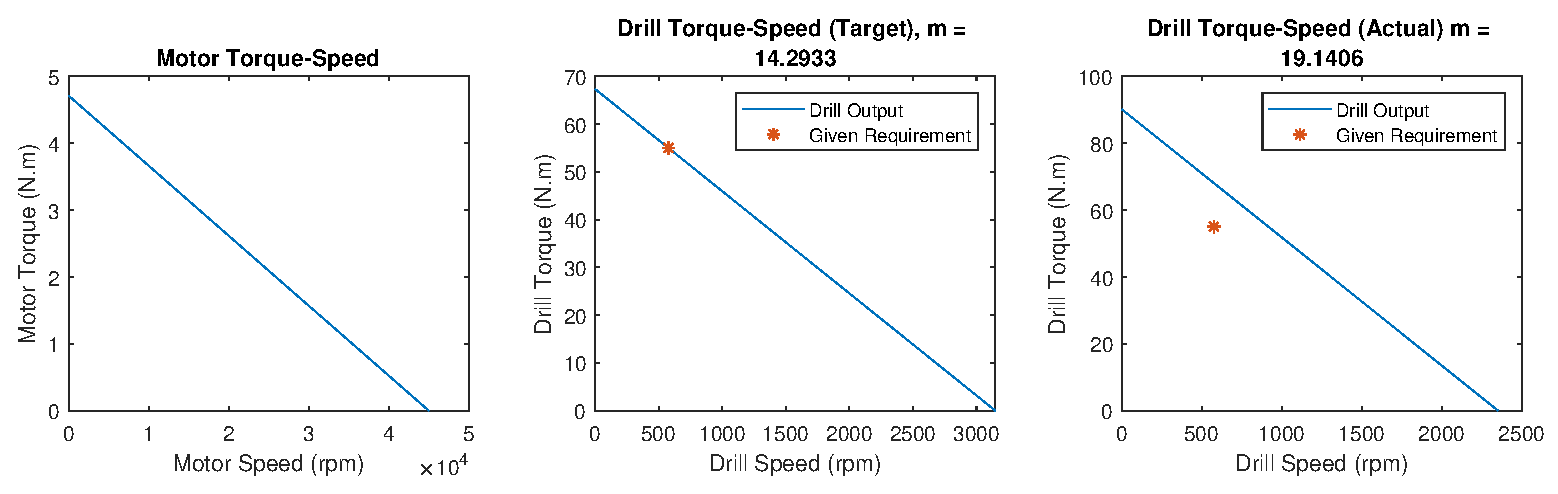
\includegraphics [width=4in]{main_03.eps}


\subsection*{Shaft Torque and Speed Estimation}

\begin{verbatim}
%{
Motor - P1  : Shaft A
N1 - P2     : Shaft B
N2 - Chuck  : Shaft C
%}

outputPower = reqOutputSpeed*reqOutputTorque*pi/30 ;
intermediatePower = outputPower/Efficiency^0.5;
inputPower = intermediatePower/Efficiency^0.5;
efficiency = outputPower/inputPower;

%Shaft C
SpeedC = reqOutputSpeed;
TorqueC = reqOutputTorque;
%Shaft B
SpeedB = SpeedC*m2actual;
TorqueB = intermediatePower/(SpeedB*pi/30);
%Shaft A
SpeedA = SpeedB*m1actual;
TorqueA = inputPower/(SpeedA*pi/30);

%Table for torque and speed estimations
TTorqueSpeedEstimation = table(TorqueA, SpeedA, TorqueB, SpeedB, TorqueC, SpeedC)

%table for power estimations
TPower = table(inputPower, intermediatePower, outputPower, efficiency)
\end{verbatim}

        \color{lightgray} \begin{verbatim}
TTorqueSpeedEstimation =

  1�1�7table

    TorqueA    SpeedA    TorqueB    SpeedB    TorqueC    SpeedC
    _______    ______    _______    ______    _______    ______

    3.1927     11006     13.251     2515.6      55        575  


TPower =

  1�1�7table

    inputPower    intermediatePower    outputPower    efficiency
    __________    _________________    ___________    __________

      3679.7           3490.9            3311.8          0.9    

\end{verbatim} \color{black}
    

\subsection*{Operating Gear Forces, Torques and Diameters}

\begin{verbatim}
%initialize arrays
Force1t = [0];
Force1r = [0];
Force2t = [0];
Force2r = [0];
P1diameter = [0];
N1diameter = [0];
P2diameter = [0];
N2diameter = [0];

for x = DiametralPitch
    x = x/0.0254;  %Teeth/inch -> teeth/meter
    P1dia = P1/x; %Teeth / (Teeth/meter) = meter
    N1dia = N1/x;
    P2dia = P2/x;
    N2dia = N2/x;

    %record diameter
    P1diameter = [P1diameter, P1dia];
    N1diameter = [N1diameter, N1dia];
    P2diameter = [P2diameter, P2dia];
    N2diameter = [N2diameter, N2dia];

    %Transmitted Load: Pinion 1 -> Gear 1 EQN 13-36
    Wt1 = (60000*inputPower*10^-3)/(pi*(P1dia*1000)*SpeedA);
    %Radial Load: Pinion 1 -> Gear 1
    Wr1 = tan(PressureAngle)*Wt1;

    %Transmitted Load: Pinion 2 -> Gear 2
    Wt2 = (60000*outputPower*10^-3)/(pi*(N2dia*1000)*SpeedC);
    %Radial Load: Pinion 2 -> Gear 2
    Wr2 = tan(PressureAngle)*Wt2;

    %Record Forces
    Force1t = [Force1t, Wt1*1000]; %kN -> N
    Force1r = [Force1r, Wr1*1000];
    Force2t = [Force2t, Wt2*1000];
    Force2r = [Force2r, Wr2*1000];
end

%Prepare arrays for table
Force1t = transpose(Force1t(2:end));
Force2t = transpose(Force2t(2:end));
Force1r = transpose(Force1r(2:end));
Force2r = transpose(Force2r(2:end));
P1diameter = transpose(P1diameter(2:end)).*100; %meters -> centimeters;
N1diameter = transpose(N1diameter(2:end)).*100; %meters -> centimeters;
P2diameter = transpose(P2diameter(2:end)).*100; %meters -> centimeters;
N2diameter = transpose(N2diameter(2:end)).*100; %meters -> centimeters;

%Table with Forces and Diameters
TForceDiameter = table(transpose(DiametralPitch), Force1t, Force1r, P1diameter, N1diameter, Force2t, Force2r, P2diameter, N2diameter)

%{

Not confident that this is correct

%Wt, Tangential Forces
Force1t = [0];
Force2t = [0];
%Wr, Radial Forces
Force1r = [0];
Force2r = [0];
%Gear Diameters
P1diameter = [0];
N1diameter = [0];
P2diameter = [0];
N2diameter = [0];
%Shaft Torques
AT = [0];
BT = [0];
CT = [0];

for x = DiametralPitch
DiametralPitch1 = x/0.0254;
DiametralPitch2 = x/0.0254;  %Teeth/inch -> teeth/meter

P1dia = P1/DiametralPitch1; %Teeth / (Teeth/meter) = meter
N1dia= N1/DiametralPitch1;
P2dia= P2/DiametralPitch2;
N2dia= N2/DiametralPitch2;

%Logging diameters for the table below
P1diameter = [P1diameter, P1dia];
N1diameter = [N1diameter, N1dia];
P2diameter = [P2diameter, P2dia];
N2diameter = [N2diameter, N2dia];

%Tangential Forces
Ctorque = CopTorque;
Wt2 = Ctorque/(cos(PressureAngle2)*N2dia/2);
Btorque = (Wt2*P2dia/2)/cos(PressureAngle2);
Wt1 = Btorque/(cos(PressureAngle1)*N1dia/2);
Atorque = (Wt1*P1dia/2)/cos(PressureAngle1);
Force2t = [Force2t, Wt2];
Force1t = [Force1t, Wt1];
%Radial Forces
Force1r = [Force1r, tan(PressureAngle1)*Wt1];
Force2r = [Force2r, tan(PressureAngle2)*Wt2];
%Shaft Torques
AT = [AT, Atorque];
BT = [BT, Btorque];
CT = [CT, Ctorque];

end

Force1t = Force1t(2:end);
Force2t = Force2t(2:end);
Force1r = Force1r(2:end);
Force2r = Force2r(2:end);

P1diameter = P1diameter(2:end);
N1diameter = N1diameter(2:end);
P2diameter = P2diameter(2:end);
N2diameter = N2diameter(2:end);

AT = AT(2:end);
BT = BT(2:end);
CT = CT(2:end);

DiametralPitch = transpose(DiametralPitch);
Force1t = transpose(Force1t);
Force2t = transpose(Force2t);
Force1r = transpose(Force1r);
Force2r = transpose(Force2r)
P1diameter = transpose(P1diameter).*100; %meters -> centimeters
N1diameter = transpose(N1diameter).*100;
P2diameter = transpose(P2diameter).*100;
N2diameter = transpose(N2diameter).*100;
AT = transpose(AT);
BT = transpose(BT);
CT = transpose(CT);

ForceTorqueTable = table(DiametralPitch, AT, Force1t, Force1r, BT,  Force2t, Force2r, CT)

DiameterTable = table(DiametralPitch, P1diameter, N1diameter, P2diameter, N2diameter)

%}
\end{verbatim}

        \color{lightgray} \begin{verbatim}
TForceDiameter =

  8�1�7table

    Var1    Force1t    Force1r    P1diameter    N1diameter    Force2t    Force2r    P2diameter    N2diameter
    ____    _______    _______    __________    __________    _______    _______    __________    __________

      8      125.7     45.751         5.08        22.225      494.94     180.14         5.08        22.225  
     10     157.12     57.188        4.064         17.78      618.67     225.18        4.064         17.78  
     12     188.55     68.626       3.3867        14.817      742.41     270.21       3.3867        14.817  
     16      251.4     91.501         2.54        11.113      989.88     360.29         2.54        11.113  
     20     314.25     114.38        2.032          8.89      1237.3     450.36        2.032          8.89  
     24      377.1     137.25       1.6933        7.4083      1484.8     540.43       1.6933        7.4083  
     32     502.79        183         1.27        5.5563      1979.8     720.57         1.27        5.5563  
     48     754.19      274.5      0.84667        3.7042      2969.6     1080.9      0.84667        3.7042  

\end{verbatim} \color{black}
    

\subsection*{Stresses}

\begin{par}
(Calculated in USCS then converted to metric)
\end{par} \vspace{1em}
\begin{verbatim}
%Init Arrays
ContactPinion1 = [0];
BendingPinion1 = [0];
ContactGear1 = [0];
BendingGear1 = [0];
ContactPinion2 = [0];
BendingPinion2 = [0];
ContactGear2 = [0];
BendingGear2 = [0];

Pinion1 = [0 0 0 0 0 0 0 0 0 0 0 0 0 0 0];
Gear1 = [0 0 0 0 0 0 0 0 0 0 0 0 0 0 0];
Pinion2 = [0 0 0 0 0 0 0 0 0 0 0 0 0 0 0];
Gear2 = [0 0 0 0 0 0 0 0 0 0 0 0 0 0 0];

for x = [1:length(DiametralPitch)]

    p1 = stresses(DiametralPitch(x), P1, SpeedA, FaceWidth(x), Force1t(x), m1actual, PressureAngle, SpeedA*Duty*60);%Speed*Duty*60 -> number of revs
    g1 = stresses(DiametralPitch(x), N1, SpeedB, FaceWidth(x), Force1t(x), m1actual, PressureAngle, SpeedB*Duty*60);
    p2 = stresses(DiametralPitch(x), P2, SpeedB, FaceWidth(x), Force2t(x), m2actual, PressureAngle, SpeedB*Duty*60);
    g2 = stresses(DiametralPitch(x), N2, SpeedC, FaceWidth(x), Force2t(x), m2actual, PressureAngle, SpeedC*Duty*60);

    Pinion1 = [Pinion1; p1];
    Gear1 = [Gear1; g1];
    Pinion2 = [Pinion2; p2];
    Gear2 = [Gear2; g2];

    if DiametralPitch(x) == DiametralPitchSelected
       PINION1 =  p1;
       GEAR1 =  g1;
       PINION2 =  p2;
       GEAR2 =  g2;
    end

end

Pinion1 = Pinion1(2:end,:);
Gear1 = Gear1(2:end,:);
Pinion2 = Pinion2(2:end,:);
Gear2 = Gear2(2:end,:);

%Appendix tables, DP varying
names = ["DP","ContactStress", "BendingStress", "ContactFOS", "BendingFOS", "Ko", "Kv", "Ks", "Km", "Kb", "Kt", "Kr", "Cf", "J", "I"];
Tpinion1 = array2table(Pinion1, 'VariableNames', names)
Tgear1 = array2table(Gear1, 'VariableNames', names)
Tpinion2 = array2table(Pinion2, 'VariableNames', names)
Tgear2 = array2table(Gear2, 'VariableNames', names)

%Prepare arrays for table
PINION1 = transpose(PINION1);
GEAR1 = transpose(GEAR1);
PINION2 = transpose(PINION2);
GEAR2 = transpose(GEAR2);

%Table for selected DP
Tselected = table(transpose(names), PINION1, GEAR1, PINION2, GEAR2)
\end{verbatim}

        \color{lightgray} \begin{verbatim}
Tpinion1 =

  8�1�7 table

    DP    ContactStress    BendingStress    ContactFOS    BendingFOS     Ko       Kv        Ks         Km      Kb    Kt    Kr    Cf     J        I   
    __    _____________    _____________    __________    __________    ____    ______    _______    ______    __    __    __    __    ____    ______

     8       198.31           8.3576          7.2734        52.846      1.25    1.4293     1.0912    1.1139    1     1     1     1     0.27    0.1308
    10       264.79             14.9          5.4473        29.642      1.25    1.3898     1.0678    1.1131    1     1     1     1     0.27    0.1308
    12       346.72           25.547          4.1601        17.288      1.25      1.36     1.0449    1.1073    1     1     1     1     0.27    0.1308
    16       516.52           56.698          2.7925        7.7897      1.25     1.317     1.0132     1.104    1     1     1     1     0.27    0.1308
    20          764           124.05          1.8879        3.5605      1.25     1.287    0.97972    1.0907    1     1     1     1     0.27    0.1308
    24       1241.9           327.75          1.1614        1.3475      1.25    1.2644    0.93489    1.0673    1     1     1     1     0.27    0.1308
    32       1855.6            731.7         0.77733       0.60361      1.25     1.232    0.90668    1.0666    1     1     1     1     0.27    0.1308
    48       3284.6           2292.7         0.43913       0.19263      1.25    1.1926    0.86806    1.0657    1     1     1     1     0.27    0.1308


Tgear1 =

  8�1�7 table

    DP    ContactStress    BendingStress    ContactFOS    BendingFOS     Ko       Kv        Ks         Km      Kb    Kt    Kr    Cf     J        I   
    __    _____________    _____________    __________    __________    ____    ______    _______    ______    __    __    __    __    ____    ______

     8        92.82           5.2751          16.879        87.814      1.25    1.4293     1.0912    1.0676    1     1     1     1     0.41    0.1308
    10       123.82           9.3871          12.653        49.347      1.25    1.3898     1.0678    1.0649    1     1     1     1     0.41    0.1308
    12       162.26           16.121          9.6551        28.735      1.25      1.36     1.0449     1.061    1     1     1     1     0.41    0.1308
    16       241.71           35.772          6.4815        12.949      1.25     1.317     1.0132    1.0577    1     1     1     1     0.41    0.1308
    20       358.75           78.799           4.367        5.8785      1.25     1.287    0.97972    1.0521    1     1     1     1     0.41    0.1308
    24       587.26           211.16          2.6677        2.1937      1.25    1.2644    0.93489    1.0442    1     1     1     1     0.41    0.1308
    32       877.42           471.37          1.7855       0.98272      1.25     1.232    0.90668    1.0434    1     1     1     1     0.41    0.1308
    48       1553.2           1477.1          1.0087       0.31361      1.25    1.1926    0.86806    1.0425    1     1     1     1     0.41    0.1308


Tpinion2 =

  8�1�7 table

    DP    ContactStress    BendingStress    ContactFOS    BendingFOS     Ko       Kv        Ks         Km      Kb    Kt    Kr    Cf     J        I   
    __    _____________    _____________    __________    __________    ____    ______    _______    ______    __    __    __    __    ____    ______

     8       363.97           28.152          4.3044         16.454     1.25    1.2227     1.0912    1.1139    1     1     1     1     0.27    0.1308
    10       488.44             50.7          3.2075         9.1367     1.25     1.201     1.0678    1.1131    1     1     1     1     0.27    0.1308
    12       642.16           87.633          2.4397          5.286     1.25    1.1848     1.0449    1.1073    1     1     1     1     0.27    0.1308
    16       962.55            196.9          1.6276         2.3526     1.25    1.1616     1.0132     1.104    1     1     1     1     0.27    0.1308
    20       1430.3           434.74          1.0954         1.0655     1.25    1.1455    0.97972    1.0907    1     1     1     1     0.27    0.1308
    24       2333.3             1157         0.67144        0.40038     1.25    1.1335    0.93489    1.0673    1     1     1     1     0.27    0.1308
    32       3505.1           2610.9         0.44696        0.17742     1.25    1.1165    0.90668    1.0666    1     1     1     1     0.27    0.1308
    48       6248.1           8296.4         0.25074       0.055835     1.25     1.096    0.86806    1.0657    1     1     1     1     0.27    0.1308


Tgear2 =

  8�1�7 table

    DP    ContactStress    BendingStress    ContactFOS    BendingFOS     Ko       Kv        Ks         Km      Kb    Kt    Kr    Cf     J        I   
    __    _____________    _____________    __________    __________    ____    ______    _______    ______    __    __    __    __    ____    ______

     8       170.36           17.769          9.9888        27.342      1.25    1.2227     1.0912    1.0676    1     1     1     1     0.41    0.1308
    10        228.4           31.941          7.4502         15.21      1.25     1.201     1.0678    1.0649    1     1     1     1     0.41    0.1308
    12       300.52           55.297          5.6623         8.786      1.25    1.1848     1.0449     1.061    1     1     1     1     0.41    0.1308
    16       450.44           124.23          3.7778        3.9109      1.25    1.1616     1.0132    1.0577    1     1     1     1     0.41    0.1308
    20        671.6           276.17          2.5337        1.7592      1.25    1.1455    0.97972    1.0521    1     1     1     1     0.41    0.1308
    24       1103.4           745.38          1.5422       0.65181      1.25    1.1335    0.93489    1.0442    1     1     1     1     0.41    0.1308
    32       1657.4             1682          1.0267       0.28885      1.25    1.1165    0.90668    1.0434    1     1     1     1     0.41    0.1308
    48       2954.6           5344.8         0.57594        0.0909      1.25     1.096    0.86806    1.0425    1     1     1     1     0.41    0.1308


Tselected =

  15�1�7table

         Var1          PINION1     GEAR1     PINION2     GEAR2 
    _______________    _______    _______    _______    _______

    "DP"                    20         20         20         20
    "ContactStress"        764     358.75     1430.3      671.6
    "BendingStress"     124.05     78.799     434.74     276.17
    "ContactFOS"        1.8879      4.367     1.0954     2.5337
    "BendingFOS"        3.5605     5.8785     1.0655     1.7592
    "Ko"                  1.25       1.25       1.25       1.25
    "Kv"                 1.287      1.287     1.1455     1.1455
    "Ks"               0.97972    0.97972    0.97972    0.97972
    "Km"                1.0907     1.0521     1.0907     1.0521
    "Kb"                     1          1          1          1
    "Kt"                     1          1          1          1
    "Kr"                     1          1          1          1
    "Cf"                     1          1          1          1
    "J"                   0.27       0.41       0.27       0.41
    "I"                 0.1308     0.1308     0.1308     0.1308

\end{verbatim} \color{black}
    

\subsection*{Torque Calculation}

\begin{verbatim}
Torque = zeros(3,1); %index 1 = Torque A, %index 2 = Torque B, %index 3 = Torque C,
Wt = zeros(4,1); %index 1 = P1, %index 2 = N1, %index 3 = P2, index 4 = N2
Wr = zeros(4,1);

Torque(3) = TorqueC;
Wt(4) = Torque(3)/(0.5*0.0254*N2/DiametralPitchSelected); %F = T/d, meters/inch* teeth / (teeth/inch)
Wr(4) = tan(PressureAngle)*Wt(4);

Torque(2) = TorqueB;
Wt(3) = Torque(2)/(0.5*0.0254*P2/DiametralPitchSelected); %F = T/d, meters/inch* teeth / (teeth/inch)
Wr(3) = tan(PressureAngle)*Wt(3);
Wt(2) = Torque(2)/(0.5*0.0254*N1/DiametralPitchSelected); %F = T/d, meters/inch* teeth / (teeth/inch)
Wr(2) = tan(PressureAngle)*Wt(2);

Torque(1) = TorqueA;
Wt(1) = Torque(1)/(0.5*0.0254*P1/DiametralPitchSelected); %F = T/d, meters/inch* teeth / (teeth/inch)
Wr(1) = tan(PressureAngle)*Wt(1);


TTorqueCalc = table(["Shaft A";"Shaft B";"Shaft C"], Torque)
TForceCalc = table(["Pinion 1";"Gear 1";"Pinion 2";"Gear 2"], Wt, Wr)
\end{verbatim}

        \color{lightgray} \begin{verbatim}
TTorqueCalc =

  3�1�7table

      Var1       Torque
    _________    ______

    "Shaft A"    3.1927
    "Shaft B"    13.251
    "Shaft C"        55


TForceCalc =

  4�1�7table

       Var1         Wt        Wr  
    __________    ______    ______

    "Pinion 1"    314.25    114.38
    "Gear 1"      298.12    108.51
    "Pinion 2"    1304.3    474.72
    "Gear 2"      1237.3    450.36

\end{verbatim} \color{black}
    

\subsection*{Shaft A BMD}

\begin{verbatim}
%define Shaft A length and positions, units: meters
LengthA = 1.5*0.0254; %inch -> meter
BearingA2pos = 1.5*0.0254;
BearingA1pos = 0; %bearing supports shaft
Motor1pos = 0; %motor generates torque
Pinion1pos = 0.5*0.0254; %inch -> meter;

pinion = [Wr(1), Wt(1), Pinion1pos, P1, 1];
gear = [0, 0, 0, 0, 0];
moment = [Torque(1), Motor1pos];
bearing = [BearingA1pos, BearingA2pos];

[OUT] = BMDGenerator(pinion, gear, bearing)
FxyA = OUT(1,:);
FxyposA = OUT(2,:);
FxzA = OUT(3,:);
FxzposA = OUT(4,:);

%Shear Force and Bending Moment Diagrams
padding = 0.2
f4 = figure('Renderer', 'painters', 'Position', [10 10 900 600])
hold on
title("Shaft A")
hold off
subplot(3,2,1)
ShearXY = Shear(LengthA, FxyposA, FxyA);
plot(ShearXY(:,1)*1000, ShearXY(:,2))
hold on
title("XY Shear Force")
xlabel("Position (mm)")
ylabel("Shear Force (N)")
hold off
subplot(3,2,2)
ShearXZ = Shear(LengthA, FxzposA, FxzA);
plot(ShearXZ(:,1)*1000, ShearXZ(:,2))
hold on
title("XZ Shear Force")
xlabel("Position (mm)")
ylabel("Shear Force (N)")
hold off
subplot(3,2,3)
BendingMomentXY = Moment(LengthA, FxyposA, FxyA);
plot(BendingMomentXY(:,1)*1000, BendingMomentXY(:,2))
hold on
title("XY Bending Moment")
xlabel("Position (mm)")
ylabel("Bending Moment (N.m)")
hold off
subplot(3,2,4)
BendingMomentXZ = Moment(LengthA, FxzposA, FxzA);
plot(BendingMomentXZ(:,1)*1000, BendingMomentXZ(:,2))
hold on
title("XZ Bending Moment")
xlabel("Position (mm)")
ylabel("Bending Moment (N.m)")
hold off
subplot(3,2,5:6)
TorqueX = TorquePlotter(LengthA, pinion, gear, moment);
plot(TorqueX(:,1)*1000, TorqueX(:,2))
hold on
title("X Torque")
xlabel("Position (mm)")
ylabel("Torque (N.m)")
hold off
\end{verbatim}

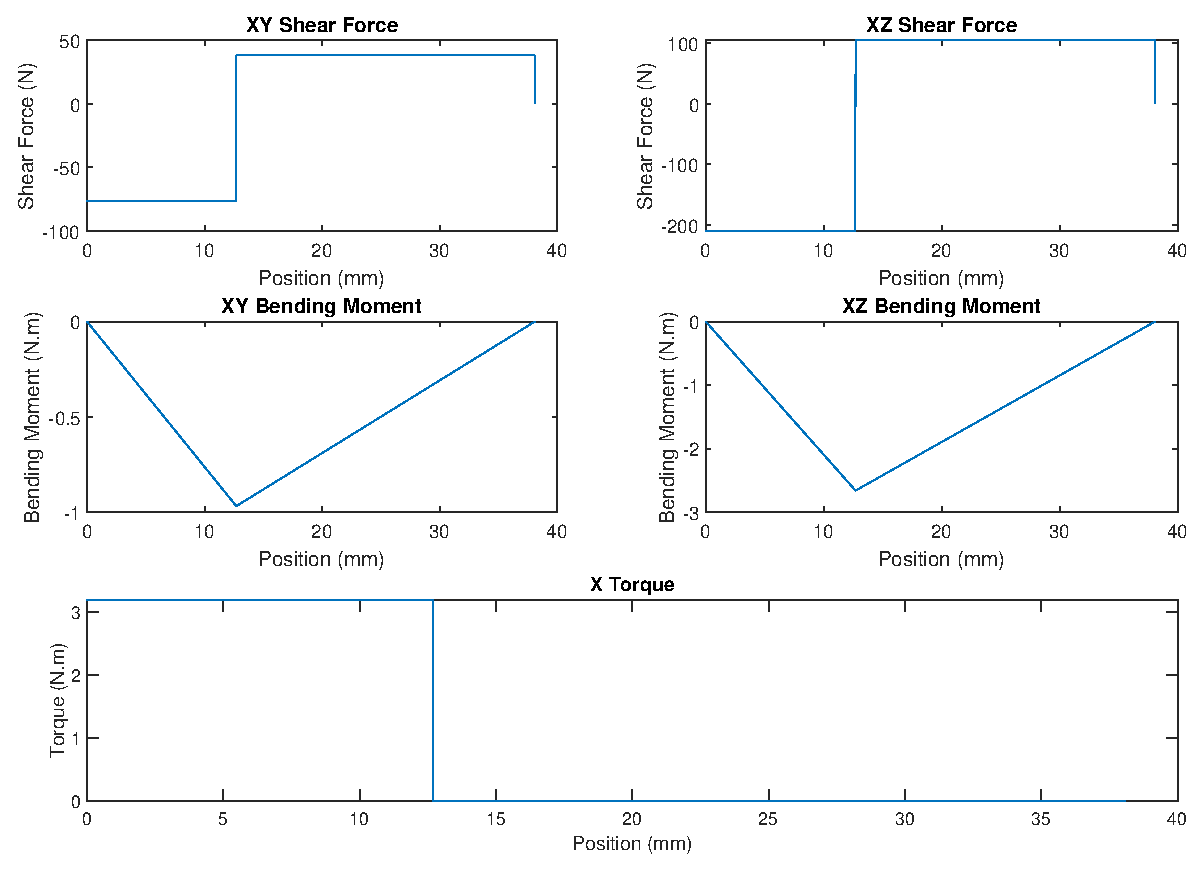
\includegraphics [width=4in]{main_04.eps}


\subsection*{Shaft B BMD}

\begin{verbatim}
%define Shaft B length and positions, units: meters
LengthB = 1.5*0.0254; %inch -> meter
BearingB2pos = 1.5*0.0254;
BearingB1pos = 0; %bearing supports shaft
Gear1pos = 0.5*0.0254; %motor generates torque
Pinion2pos = 1*0.0254; %inch -> meter;

pinion = [Wr(3), Wt(3), Pinion2pos, P2, 1];
gear = [ Wr(2), Wt(2), Gear1pos, N1, 0];
moment = [0, 0];
bearing = [BearingB1pos, BearingB2pos];

[OUT] = BMDGenerator(pinion, gear, bearing)
FxyB = OUT(1,:);
FxyposB = OUT(2,:);
FxzB = OUT(3,:);
FxzposB = OUT(4,:);

%Shear Force and Bending Moment Diagrams
padding = 0.2
f5 = figure('Renderer', 'painters', 'Position', [10 10 900 600])
hold on
title("Shaft B")
hold off
subplot(3,2,1)
ShearXY = Shear(LengthB, FxyposB, FxyB);
plot(ShearXY(:,1)*1000, ShearXY(:,2))
hold on
title("XY Shear Force")
xlabel("Position (mm)")
ylabel("Shear Force (N)")
hold off
subplot(3,2,2)
ShearXZ = Shear(LengthB, FxzposB, FxzB);
plot(ShearXZ(:,1)*1000, ShearXZ(:,2))
hold on
title("XZ Shear Force")
xlabel("Position (mm)")
ylabel("Shear Force (N)")
hold off
subplot(3,2,3)
BendingMomentXY = Moment(LengthB, FxyposB, FxyB);
plot(BendingMomentXY(:,1)*1000, BendingMomentXY(:,2))
hold on
title("XY Bending Moment")
xlabel("Position (mm)")
ylabel("Bending Moment (N.m)")
hold off
subplot(3,2,4)
BendingMomentXZ = Moment(LengthB, FxzposB, FxzB);
plot(BendingMomentXZ(:,1)*1000, BendingMomentXZ(:,2))
hold on
title("XZ Bending Moment")
xlabel("Position (mm)")
ylabel("Bending Moment (N.m)")
hold off
subplot(3,2,5:6)
TorqueX = TorquePlotter(LengthB, pinion, gear, moment);
plot(TorqueX(:,1)*1000, TorqueX(:,2))
hold on
title("X Torque")
xlabel("Position (mm)")
ylabel("Torque (N.m)")
hold off
\end{verbatim}

        \color{lightgray} \begin{verbatim} 
SigmaFxy =
 
B1xy + B2xy + 2565049596265321/4398046511104 == 0
 
 
SigmaMxy =
 
(381*B2xy)/10000 + 60509782446090171/4503599627370496 == 0
 
 
SigmaFxz =
 
B1xz + B2xz + 7047415845520165/4398046511104 == 0
 
 
SigmaMxz =
 
(381*B2xz)/10000 + 41562315231686103/1125899906842624 == 0
 
 
eqns =
 
          B1xy + B2xy + 2565049596265321/4398046511104 == 0
 (381*B2xy)/10000 + 60509782446090171/4503599627370496 == 0
          B1xz + B2xz + 7047415845520165/4398046511104 == 0
 (381*B2xz)/10000 + 41562315231686103/1125899906842624 == 0
 

soln = 

  struct with fields:

    B1xy: [1�1�7sym]
    B1xz: [1�1�7sym]
    B2xy: [1�1�7sym]
    B2xz: [1�1�7sym]


soln =

 -230.5772
 -633.5057
 -352.6475
 -968.8911


OUT =

   1.0e+03 *

   -0.2306    0.4747    0.1085   -0.3526
         0    0.0000    0.0000    0.0000
   -0.6335    1.3043    0.2981   -0.9689
         0    0.0000    0.0000    0.0000


padding =

    0.2000


f5 = 

  Figure (3) with properties:

      Number: 3
        Name: ''
       Color: [0.9400 0.9400 0.9400]
    Position: [10 10 900 600]
       Units: 'pixels'

  Use GET to show all properties


t =

     0


t =

   13.2514


t =

  -13.2514

\end{verbatim} \color{black}
    
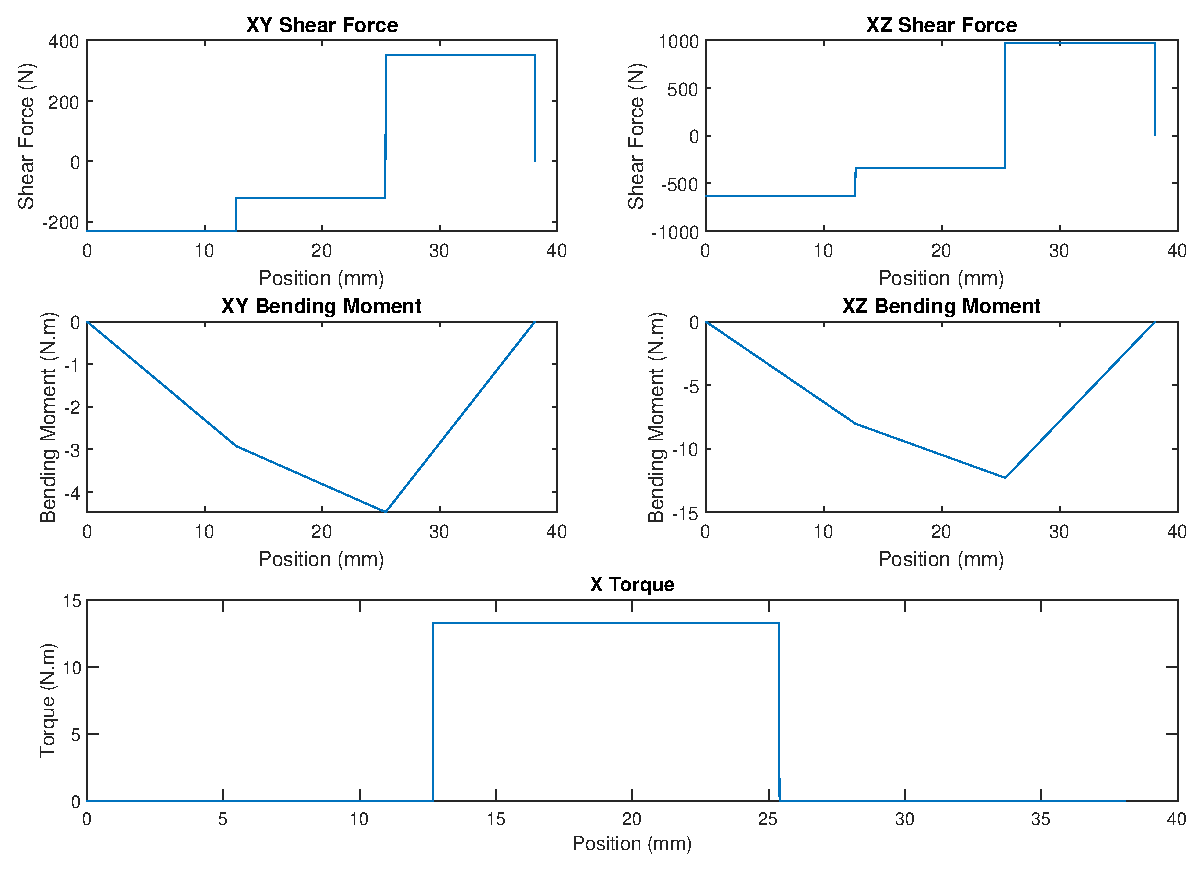
\includegraphics [width=4in]{main_05.eps}


\subsection*{Shaft C BMD}

\begin{verbatim}
%define Shaft B length and positions, units: meters
LengthC = 1.5*0.0254; %inch -> meter
BearingC2pos = 1*0.0254;
BearingC1pos = 0; %bearing supports shaft
Gear2pos = 0.5*0.0254; %motor generates torque
Chuckpos = 1.5*0.0254; %inch -> meter;

pinion = [0,0,0,0,0];
gear = [Wr(4), Wt(4), Gear2pos, N2, 0];
moment = [-1*Torque(3), Chuckpos];
bearing = [BearingC1pos, BearingC2pos];

[OUT] = BMDGenerator(pinion, gear, bearing)
FxyC = OUT(1,:);
FxyposC = OUT(2,:);
FxzC = OUT(3,:);
FxzposC = OUT(4,:);

%Shear Force and Bending Moment Diagrams
padding = 0.2
f6 = figure('Renderer', 'painters', 'Position', [10 10 900 600])
hold on
title("Shaft C")
hold off
subplot(3,2,1)
ShearXY = Shear(LengthC, FxyposC, FxyC);
plot(ShearXY(:,1)*1000, ShearXY(:,2))
hold on
title("XY Shear Force")
xlabel("Position (mm)")
ylabel("Shear Force (N)")
hold off
subplot(3,2,2)
ShearXZ = Shear(LengthC, FxzposC, FxzC);
plot(ShearXZ(:,1)*1000, ShearXZ(:,2))
hold on
title("XZ Shear Force")
xlabel("Position (mm)")
ylabel("Shear Force (N)")
hold off
subplot(3,2,3)
BendingMomentXY = Moment(LengthC, FxyposC, FxyC);
plot(BendingMomentXY(:,1)*1000, BendingMomentXY(:,2))
hold on
title("XY Bending Moment")
xlabel("Position (mm)")
ylabel("Bending Moment (N.m)")
hold off
subplot(3,2,4)
BendingMomentXZ = Moment(LengthC, FxzposC, FxzC);
plot(BendingMomentXZ(:,1)*1000, BendingMomentXZ(:,2))
hold on
title("XZ Bending Moment")
xlabel("Position (mm)")
ylabel("Bending Moment (N.m)")
hold off
subplot(3,2,5:6)
TorqueX = TorquePlotter(LengthC, pinion, gear, moment);
plot(TorqueX(:,1)*1000, TorqueX(:,2))
hold on
title("X Torque")
xlabel("Position (mm)")
ylabel("Torque (N.m)")
hold off
\end{verbatim}

        \color{lightgray} \begin{verbatim} 
SigmaFxy =
 
B1xy + B2xy + 7922761848621797/17592186044416 == 0
 
 
SigmaMxy =
 
(127*B2xy)/5000 + 1609905207639949/281474976710656 == 0
 
 
SigmaFxz =
 
B1xz + B2xz + 5441902319701237/4398046511104 == 0
 
 
SigmaMxz =
 
(127*B2xz)/5000 + 110/7 == 0
 
 
eqns =
 
      B1xy + B2xy + 7922761848621797/17592186044416 == 0
 (127*B2xy)/5000 + 1609905207639949/281474976710656 == 0
       B1xz + B2xz + 5441902319701237/4398046511104 == 0
                            (127*B2xz)/5000 + 110/7 == 0
 

soln = 

  struct with fields:

    B1xy: [1�1�7sym]
    B1xz: [1�1�7sym]
    B2xy: [1�1�7sym]
    B2xz: [1�1�7sym]


soln =

 -225.1784
 -618.6727
 -225.1784
 -618.6727


OUT =

   1.0e+03 *

   -0.2252         0    0.4504   -0.2252
         0         0    0.0000    0.0000
   -0.6187         0    1.2373   -0.6187
         0         0    0.0000    0.0000


padding =

    0.2000


f6 = 

  Figure (4) with properties:

      Number: 4
        Name: ''
       Color: [0.9400 0.9400 0.9400]
    Position: [10 10 900 600]
       Units: 'pixels'

  Use GET to show all properties


t =

     0


t =

    55


t =

   -55

\end{verbatim} \color{black}
    
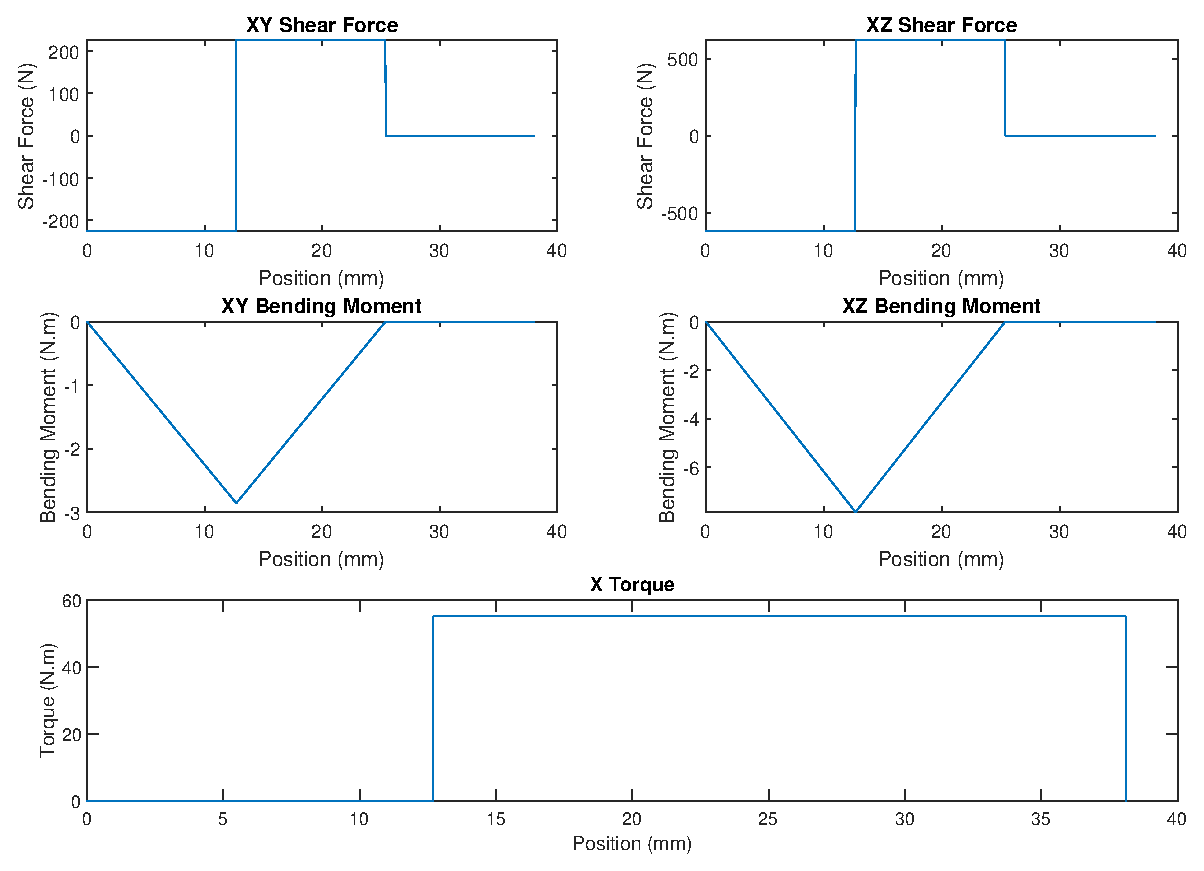
\includegraphics [width=4in]{main_06.eps}


\subsection*{BMD Tables}



\subsection*{Endurance Limits}

\begin{verbatim}
%Shaft Daimeters (meters) 1 = A, 2 = B...
Diameters = [5*10^-3; 5*10^-3; 5*10^-3];

%Shaft Material Properties
%Ultimate Tensile Stress (MPa)
UltimateTensile = [800; 800; 800]; %assumed material from CES

%Endurance Limits (MPa)
EA = enduranceLimit(Diameters(1), UltimateTensile(1));
EB = enduranceLimit(Diameters(2), UltimateTensile(2));
EC = enduranceLimit(Diameters(3), UltimateTensile(3));
EnduranceLimit = [EA(1); EB(1); EC(1)];
MarinFactors = [EA; EB; EC];

TEnduranceLimit = table(Diameters, UltimateTensile, EnduranceLimit)
TMarinFactors = array2table([["A";"B";"C"],Diameters, UltimateTensile, MarinFactors], 'VariableNames', ["Shaft","Diameters","UltimateTensile","EnduranceLimit","Ka","Kb","Kc","Kd","Ke","Kf"])
\end{verbatim}

        \color{lightgray} \begin{verbatim}
kb =

    1.0461


kc =

     1


kb =

    1.0461


kc =

     1


kb =

    1.0461


kc =

     1


TEnduranceLimit =

  3�1�7table

    Diameters    UltimateTensile    EnduranceLimit
    _________    _______________    ______________

      0.005            800              261.79    
      0.005            800              261.79    
      0.005            800              261.79    


TMarinFactors =

  3�1�7 table

    Shaft    Diameters    UltimateTensile    EnduranceLimit        Ka             Kb        Kc        Kd         Ke       Kf 
    _____    _________    _______________    ______________    ___________    __________    ___    ________    _______    ___

     "A"      "0.005"          "800"           "261.7855"      "0.7671101"    "1.046115"    "1"    "1.0019"    "0.814"    "1"
     "B"      "0.005"          "800"           "261.7855"      "0.7671101"    "1.046115"    "1"    "1.0019"    "0.814"    "1"
     "C"      "0.005"          "800"           "261.7855"      "0.7671101"    "1.046115"    "1"    "1.0019"    "0.814"    "1"

\end{verbatim} \color{black}
    

\subsection*{Test}

\begin{verbatim}
%{
L = 61
Fpos = [0 14 34 49 61]
F = [82.24 -80 -110 142.76 -35]
figure()
subplot(2,1,1)
plot(Shear(L, Fpos, F))
subplot(2,1,2)
plot(Moment(L, Fpos, F))
%}

function [OUTPUT] = BMDGenerator(pinion, gear, bearing)

Pxy = pinion(1);
Pxz = pinion(2);
PPos = pinion(3);
P = pinion(4);

Gxy = gear(1);
Gxz = gear(2);
GPos = gear(3);
N = gear(4);

B1Pos = bearing(1);
B2Pos = bearing(2);

DiametralPitchSelected = 20;
%generate system of equations for the shaft
% Variable naming convention: B1xy
% B = Bearing, P = Pinion, G = Gear, M = motor or chuck
% 1 = first bearing from the origin, 2 = second from origin...
% xy, xz, yz = reference plane
% Prad = pinion radius, Grad = gear radius
syms B1xy B1xz B2xy B2xz

Prad = 0.5*0.0254*P/DiametralPitchSelected;
Grad = 0.5*0.0254*N/DiametralPitchSelected;

% xy equations
SigmaFxy = B1xy + B2xy + Pxy + Gxy == 0
SigmaMxy = B1xy*B1Pos + B2xy*B2Pos + Pxy*PPos + Gxy*GPos == 0

% xz equations
SigmaFxz = B1xz + B2xz + Pxz + Gxz == 0
SigmaMxz = B1xz*B1Pos + B2xz*B2Pos + Pxz*PPos + Gxz*GPos == 0

%Solve system of equations
eqns = [SigmaFxy; SigmaMxy; SigmaFxz; SigmaMxz]
soln = solve(eqns)
soln = structfun(@double,soln)

%define bearing values
B1xy = soln(1);
B1xz = soln(2);
B2xy = soln(3);
B2xz = soln(4);

Fxypos = [B1Pos, PPos, GPos, B2Pos];
Fxzpos = [B1Pos, PPos, GPos, B2Pos];
Fxy = [B1xy, Pxy, Gxy, B2xy];
Fxz = [B1xz, Pxz, Gxz, B2xz];

OUTPUT = [Fxy; Fxypos; Fxz; Fxzpos];
end

%Shear Force Diagram Plotter: Tlength = length of shaft, Fpos = array of force
%positions (3 decimal places or fewer), F = array for force vectors (Transverse Direction Only)
function V = Shear(Tlength, FPos, F)
    RES = 10^-6; %
    size = ceil(Tlength/RES + 1);
    V = zeros(size, 2); %array which shear is plotted
    k = 0;
    for i = 1:length(FPos)
        k = k+1;
        v = F(k);
        for pos = 0:RES:Tlength
            index = int64((pos/RES)+1);
            V(index, 1) = pos;
            if(pos >= FPos(i))
                V(index, 2) = V(index, 2) + v;
            end
        end
    end
end

%Bending Moment Plotter: Tlength = length of shaft, Fpos = array of force
%positions (3 decimal places or fewer), F = array for force vectors (Transverse Direction Only)
function M = Moment(Tlength, FPos, F)
    RES = 10^-6;
    size = ceil(Tlength/RES + 1);
    M = zeros(size, 2);
    k = 0;
    for i = 1:length(FPos)
        k = k+1;
        mx = F(k);
        for pos = 0:RES:Tlength
            index = int64((pos/RES)+1);
            M(index, 1) = pos;
            if(pos >= FPos(i))
                M(index, 2) = M(index, 2) + mx*(pos - FPos(i));
            end
        end
    end
end

%Bending Moment Plotter: Tlength = length of shaft, Fpos = array of force
%positions (3 decimal places or fewer), F = array for force vectors (Transverse Direction Only)
function T = TorquePlotter(Tlength, pinion, gear, moment)
    DiametralPitchSelected = 20;
    RES = 10^-6;
    size = ceil(Tlength/RES + 1);
    T = zeros(size, 2);

    Pxz = pinion(2);
    PPos = pinion(3);
    P = pinion(4);
    Prad = 0.5*0.0254*P/DiametralPitchSelected;
    Pdir = pinion(5);
    if Pdir == 1
        Pxz = Pxz*-1;
    end


    Gxz = gear(2);
    GPos = gear(3);
    N = gear(4);
    Grad = 0.5*0.0254*N/DiametralPitchSelected;
    Gdir = gear(5);
    if Gdir == 1
        Gxz = Gxz*-1;
    end

    Myz = moment(1);
    Mpos = moment(2);

    ActingTorques = [Myz, Mpos; Gxz*Grad, GPos; Pxz*Prad, PPos];
    ActingTorques = sortrows(ActingTorques, 2); %sort by position

    k = 0;
    for i = 1:length(ActingTorques)
        k = k+1;
        t = ActingTorques(k,1)
        for pos = 0:RES:Tlength
            index = int64((pos/RES)+1);
            T(index, 1) = pos;
            if(pos >= ActingTorques(i,2))
                T(index, 2) = T(index, 2) + t;
            end
        end
    end
end

%{
Pd = Diametral Pitch (teeth/inch)
N = Number of Teeth
n = Angular Velocity (rpm)
F = Face Width (inches)
WtM = Tangetntial load (Newtons)
m = gear Ratio
phi = pressure angle (Rad)
duty = number of revs
%}
function [OUTPUT] = enduranceLimit(shaftDiameter, Sut)
    %SI Units

    if Sut <= 1400 %Eq. 6-8
        Se_ = 0.5*Sut;
    else
        Se_ = 700;
    end

    %Ka - surface condition factor
    a = 4.51; %Machined/CD, T6-2
    b = -0.265; %T6-2
    ka = a*Sut^b; %Eq. 6-19

    %Kb - size modification factor
    d = shaftDiameter*10^3; %mm
    if d <= 51 %Eq. 6-20
        kb = (d/7.62)^-0.107
    else
        kb = 1.51*d^-0.157
    end

    %Kc - load mofification factor
    kc = 1% Eq. 6-26, Bending

    %Kd - temperature modification factor
    Tf = 77; % room temp in degF, 25 degC
    kd = 0.975 + Tf*0.432*10^-3 - Tf^2*0.115*10^-5 + Tf^3*0.104*10^-8 - Tf^4*0.595*10^-12; %Eq. 6-27

    %Ke - reliability factir
    ke = 0.814; %T6-5, 99% reliability

    %Kf - misc effects modification factor
    kf = 1;

    Se = ka*kb*kc*kd*ke*kf*Se_;

    OUTPUT = [Se, ka, kb, kc, kd, ke, kf];
end


%{
Pd = Diametral Pitch (teeth/inch)
N = Number of Teeth
n = Angular Velocity (rpm)
F = Face Width (inches)
WtM = Tangetntial load (Newtons)
m = gear Ratio
phi = pressure angle (Rad)
duty = number of revs
%}
function [OUTPUT] = stresses(Pd, N, n, F, WtM, m, phi, duty)
    dp = N/Pd;             %Diameter inches
    V = pi*dp*n/12;        %Linear Velocity
    Wt = 0.224809*WtM ;     % Newtons -> lbf


    %Ko - Overload Factor
    Ko = 1.25; %uniform - MODERATE SHOCK

    %Kv - Dynamic Factor
    Qv = 9; %Low end of precision quality gears, Catalog: pg. 48, AGMA class: 9
    B = 0.25*(12 - Qv)^(2/3);
    A = 50 + 56*(1 - B);
    Kv = ((A + V^0.5)/A)^B;

    %Ks - Size Factor
    x = 1.5708/Pd; %Tooth Width, equation from boston
    Y = 2*x*Pd/3;
    Ks = 1.192*((F*Y^0.5)/Pd)^0.0535;

    %Km - Load Distribution Factor
    Cmc = 0.8; %Crowned
    Cpf = F/(10*dp) - 0.025;
    Cpm = 1;
    A = 0.0675; %PRECISION, enclosed, Table 14-9
    B = 0.0167;
    C = -0.926E-4;
    Cma = A + B*F + C*F^2;
    Ce = 1;
    Km = 1 + Cmc*(Cpf*Cpm + Cma*Ce);

    %Kb - Rim Thickness Factor
    Kb = 1; %Assumption given by professor
    %{
    if Pd < 20 %Whole Depth Equation from Boston
        ht = 2.157/Pd;
    else
        ht = 2.2/Pd + 0.002;
    end

    tr = %Cannot find equation or values specifying rim thickness

    mb = tr/ht;
    if mb < 1.2
        Kb = 1.6*log(2.242/mb);
    else
        Kb = 1;
    end
    %}

    %J - Bending Strength Geometry Factor Fig. 14-6, Very bad lookup table
    %for selected gears
    if N == 16
        J = 0.27;
    else
        J = 0.41;
    end

    %Kt - Temperature Factor
    Kt = 1; %Less than 250F

    %Kr - Reliability Factor
    Kr = 1; %0.99 - Eq. 14-38

    %Cp - Elastic Coefficient
    Cp = 2300; %Table 14-8 steel-steel

    %I - Pitting Resistance Geometry Factor
    mn = 1; %Load sharing ratio: 1 for spur gears
    I = ((cos(phi)*sin(phi))/(2*mn))*(m/(m+1));

    %Cf - surface condition factor
    Cf = 1;

    %Contact Stress
    CS = (Cp*sqrt(Wt*Ko*Kv*Ks*(Km/(dp*F))*(Cf/I))); %Contact stress in psi

    %Bending Stress
    BS = (Wt*Ko*Kv*Ks*(Pd/F)*((Km*Kb)/J)); %Contact stress in psi

    %Factor of Safety

    %Table 14-6, Grade 3 steel, carburized and hardened
    St = 75000;
    Sc = 275000; %psi

    if duty > 10^4 %Fig 14-15
        Zn = 2.466*duty^-0.056;
    else
        Zn = 1.5;
    end

    Ch = 1;

    if duty > 10^6 %Fig 14-14
        Yn = 1.6831*duty^-0.0323;
    else
        Yn = 6.1514*duty^-0.1192;
    end

    %Contact FOS
    CFOS = ((Sc*Zn*Ch)/(Kt*Kr))/CS;

    %Bending FOS
    BFOS = ((St*Yn)/(Kt*Kr))/BS;

    CS = CS*0.00689476; %psi -> MPa
    BS = BS*0.00689476;

    OUTPUT = [Pd, CS, BS, CFOS, BFOS, Ko, Kv, Ks, Km, Kb, Kt, Kr, Cf, J, I];
end
\end{verbatim}

        \color{lightgray} \begin{verbatim} 
SigmaFxy =
 
B1xy + B2xy + 8048519973203097/70368744177664 == 0
 
 
SigmaMxy =
 
(381*B2xy)/10000 + 6541837034219477/4503599627370496 == 0
 
 
SigmaFxz =
 
B1xz + B2xz + 2764140860800629/8796093022208 == 0
 
 
SigmaMxz =
 
(381*B2xz)/10000 + 1760/441 == 0
 
 
eqns =
 
        B1xy + B2xy + 8048519973203097/70368744177664 == 0
 (381*B2xy)/10000 + 6541837034219477/4503599627370496 == 0
         B1xz + B2xz + 2764140860800629/8796093022208 == 0
                          (381*B2xz)/10000 + 1760/441 == 0
 

soln = 

  struct with fields:

    B1xy: [1�1�7sym]
    B1xz: [1�1�7sym]
    B2xy: [1�1�7sym]
    B2xz: [1�1�7sym]


soln =

  -76.2509
 -209.4976
  -38.1254
 -104.7488


OUT =

  -76.2509  114.3763         0  -38.1254
         0    0.0127         0    0.0381
 -209.4976  314.2464         0 -104.7488
         0    0.0127         0    0.0381


padding =

    0.2000


f4 = 

  Figure (2) with properties:

      Number: 2
        Name: ''
       Color: [0.9400 0.9400 0.9400]
    Position: [10 10 900 600]
       Units: 'pixels'

  Use GET to show all properties


t =

    3.1927


t =

     0


t =

   -3.1927

\end{verbatim} \color{black}
    


\end{document}
    
